\documentclass[byrevtex,amssymb,aps,pra,floatfix,letterpaper]{revtex4}
\usepackage{graphicx}
\usepackage{hyperref}
\usepackage{subfigure}
\usepackage{amsmath}
\bibliographystyle{apsrev}
\date{\today}
\pagestyle{plain}
\newcommand{\degree}[0]{$^\circ$}

\begin{document}

\title{Experiment 4: Gas phase IR spectroscopy (HCl)}

\date{\today}

\maketitle

\section{Introduction}

Infrared (IR) spectroscopy is a powerful optical method for detecting vibrational and rotational modes of molecules. The rotational modes are usually only visible in the gas phase. A typical application of IR spectroscopy is to identify unknown molecules, to determine their concentrations and to study bond strengths in molecules. For identifying purposes, most spectrometers include a database of IR spectra and, for small molecules, an on-line database have been compiled \cite{webbook}. For molecules in the gas phase, IR spectroscopy also provides important information about molecular structure. For an overview of gas phase IR spectroscopy, see Refs. \cite{SILBEY,ATKINS1,HERZBERG1,HERZBERG2}. The latter two references also contain an extensive compilation of reference data. In this experiment, vibration-rotation spectrum of HCl molecule in the gas phase will be studied. Analysis of the experimental spectrum provides, for example, information about the H -- Cl bond length and the rotational temperature.

\section{Theory}

If electromagnetic radiation (i.e., here IR photons) is in resonance with vibration-rotation transition of a molecule, absorption of the photon occurs and the molecule becomes vibrationally and rotationally excited. In IR spectroscopy, the photon energies are typically between 200 -- 4000 cm$^{-1}$. In order to understand the origin of an IR spectrum, the energy levels and selection rules between the levels must be established. In general, we can divide the consideration into electronic, vibrational and rotational degrees of freedom because the corresponding transitions are located far away from each other and the overall Hamiltonian can be separated (approximation). In IR spectroscopy, electronic transitions are not excited and therefore we don't need to consider it further here. It should be noted, however, that sometimes under special circumstances, it is possible to observe resolved vibrational and rotational structure in UV/VIS spectra as well.

For a diatomic molecule, such as HCl, we can approximate the interaction between the atoms by the harmonic potential ($HO$):

\begin{equation}
V_{HO}(r) = \frac{1}{2}k\left(r - r_e\right)^2
\label{eq1}
\end{equation}

\noindent
where $k$ is the force constant describing stiffness of the bond, $r$ is the distance between the atoms and $r_e$ is the equilibrium bond length. A plot of Eq. (\ref{eq1}) with ``small'' and ``large'' values of $k$ are shown in Fig. \ref{fig1}. A graphical comparison between the harmonic potential $V_{HO}$ and the true potential between the atoms is demonstrated in Fig. \ref{fig1}. Through the Taylor series expansion, it can be shown that the force constant is related to the true potential $V$ at $r_e$ by:

\begin{equation}
k = \left(\frac{\partial V}{\partial r}\right)_{r = r_e}
\label{eq2}
\end{equation}

\noindent
This shows that the force constant $k$ tells us how rapidly the potential changes around the equilibrium bond length (``stiffness of the bond'').

\begin{figure}[!h]
\begin{center}
\subfigure{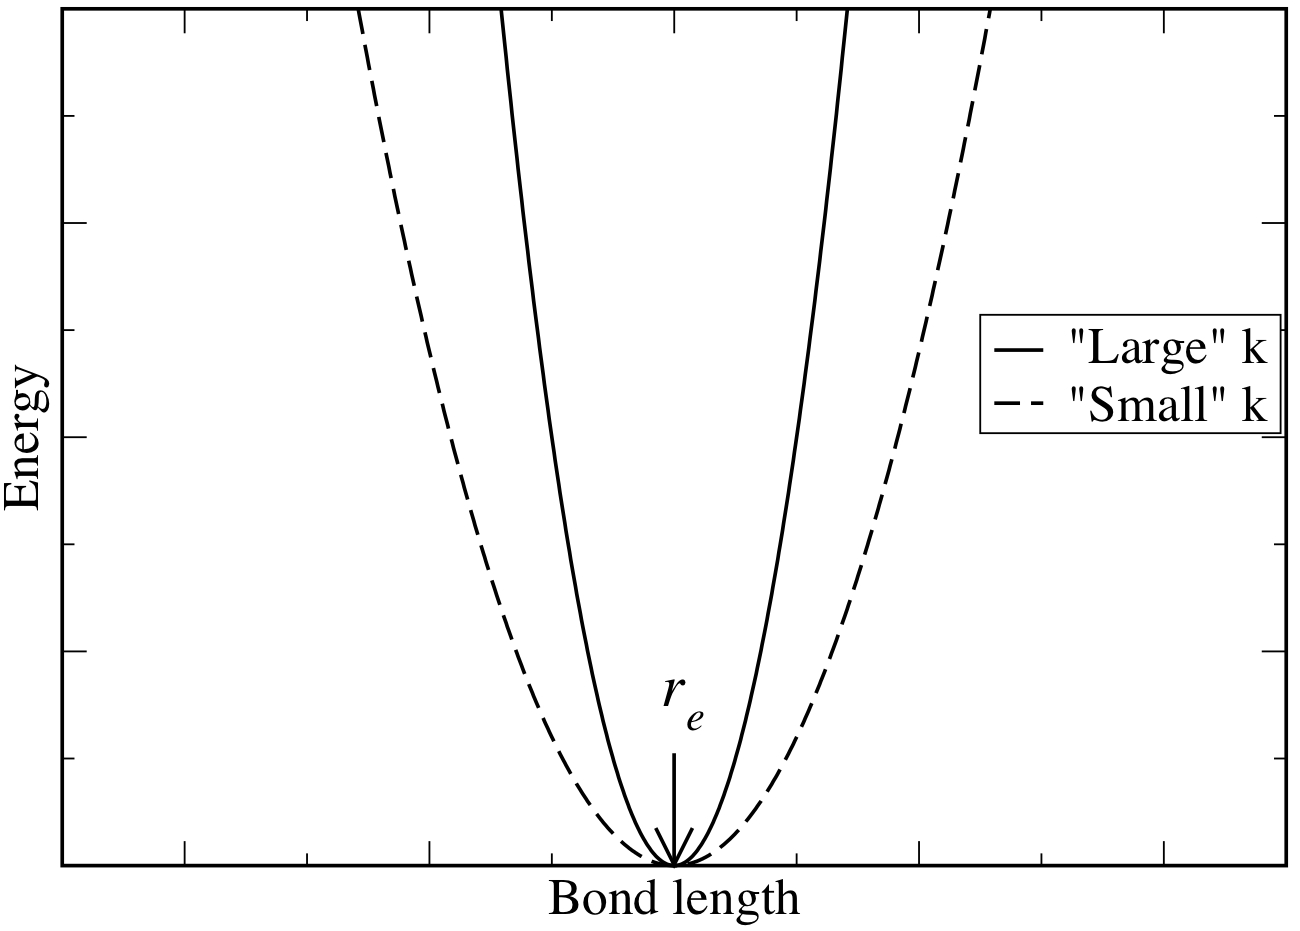
\includegraphics[scale=0.4]{fig1a}}
\subfigure{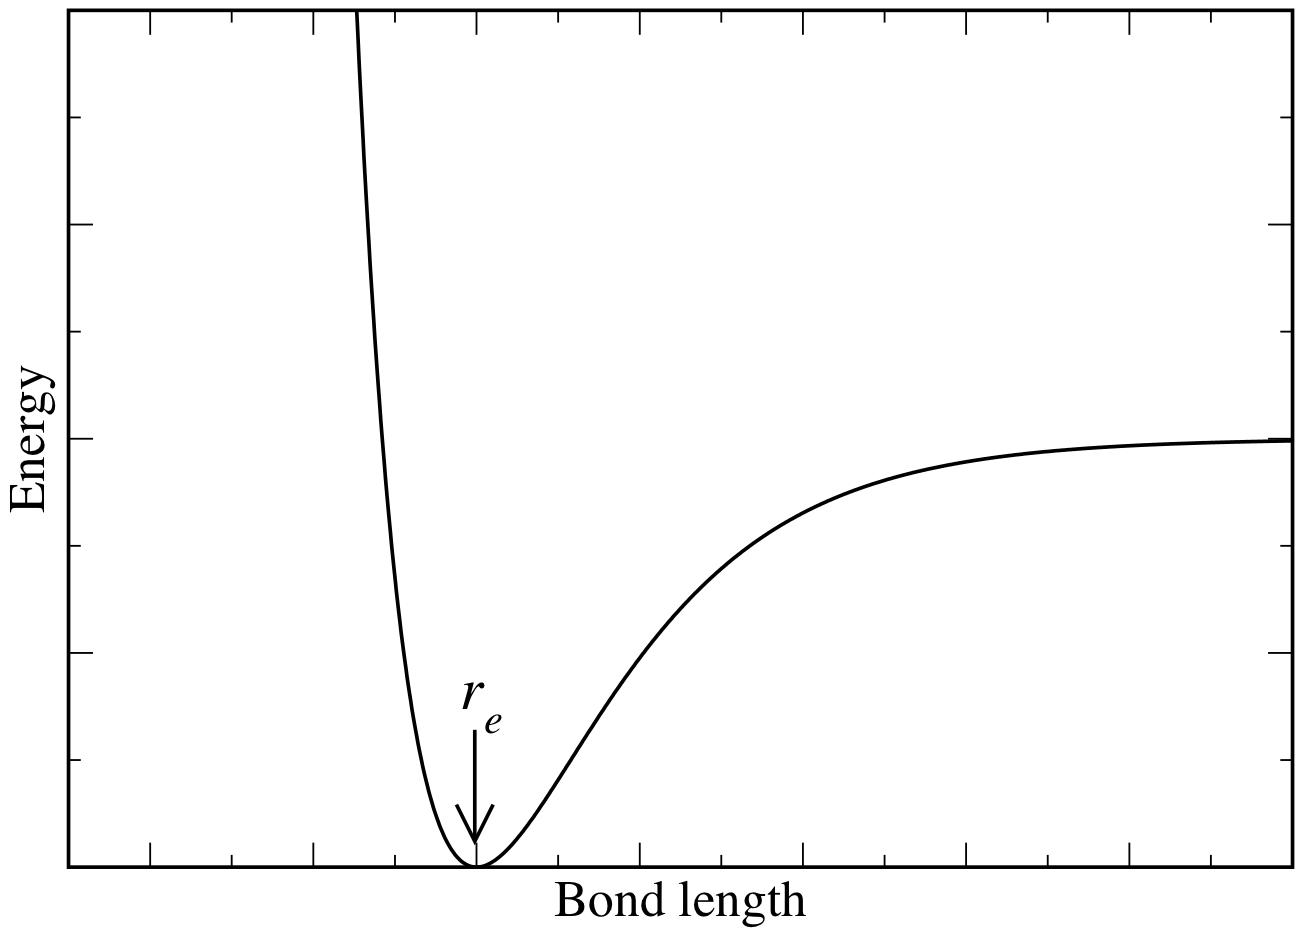
\includegraphics[scale=0.4]{fig1b}}
\end{center}
\caption{Plots of harmonic potentials with two different values of $k$ are shown on the left. A plot of Morse potential, which resembles more the ``true pair potential'', is given on the right. Note that the Morse potential allows for dissociation of the molecule whereas the harmonic potential does not.}
\label{fig1}
\end{figure}

The Schr\"odinger equation for vibration of a diatomic molecule is (one dimensional equation):

\begin{equation}
-\frac{\hbar^2}{2\mu}\frac{d^2\psi_v(r)}{dr^2} + \frac{1}{2}k(r - r_e)^2\psi_v(r) = E_v\psi_v(r)
\label{eq3}
\end{equation}

\noindent
where $\hbar$ is the Planck's constant (1.0545727 $\times$ 10$^{-34}$ Js), $\psi_v$ is the vibronic wavefunction for state $v$, $E_v$ is the energy of vibronic level $v$, and $\mu$ is the reduced mass given by:

\begin{equation}
\mu = \frac{m_1 m_2}{m_1 + m_2}
\label{eq4}
\end{equation}

\noindent
with $m_1$ being the mass of atom 1 (for example, H) and $m_2$ the mass of atom 2 (for example, Cl). The solutions to Eq. (\ref{eq3}) are given by \cite{ATKINS1,HERZBERG1}:

\begin{equation}
E_v = \left(v + \frac{1}{2}\right)\hbar\omega\textnormal{ with }\omega = \sqrt{k/\mu}\textnormal{ and }v = 0,1,2,3,...
\label{eq5}
\end{equation}

\noindent
where $v$ is the vibrational quantum number. In wavenumber energy units (m$^{-1}$; `` $\tilde{~}$ '' reminds us about the wavenumber units; most often used as cm$^{-1}$), which are usually used in IR spectroscopy, this equation reads:

\begin{equation}
\tilde{E}_v = \left(v + \frac{1}{2}\right)\tilde{\nu}\textnormal{ where }\tilde{\nu} = \frac{1}{2\pi c}\sqrt{\frac{k}{\mu}}
\label{eq6}
\end{equation}

\noindent
where $\tilde{E}_v$ is the energy in wavenumber units and $c$ is the speed of light (2.99792458 $\times$ 10$^8$ m/s). Note that Cl atoms have two isotopes (76\% of $^{35}$Cl and 24\% of $^{37}$Cl), which have different masses. For example, an ensemble of HCl molecules should display two different vibrational species in its vibrational spectrum. The eigenfunctions for the lowest vibrational levels can be written as:

\begin{equation}
\psi_0 \propto e^{-x^2/\alpha^2}\textnormal{ and }\psi_1 \propto xe^{-x^2/\alpha^2}\textnormal{ where }\alpha = \left(\frac{\hbar^2}{\mu k}\right)^{1/4}
\label{eq7}
\end{equation}

\noindent
For an IR allowed transition, the following integral must be non-zero (``the Fermi golden rule'') \cite{ATKINS2}:

\begin{equation}
I \propto \left|\left<\psi_i\left|H_1\right|\psi_f\right>\right|^2 = \left|\int\psi_i^*H_1\psi_fd\tau\right|^2
\label{eq8}
\end{equation}

\noindent
where $I$ denotes the IR transition intensity, $\psi_i$ is the wavefunction for the initial state, $\psi_f$ is the wavefunction for the final state and $H_1$ is the transition dipole operator corresponding to the electromagnetic field. For a photon absorption process, the operator $H_1$ is in general either $x$, $y$, or $z$ (i.e., multiplication by the coordinate). However, here we take just one of them (denoted by $r$), which happens to lie along molecular axis (i.e., diatomic molecule assumed). In the present case, thermal energies are only able to populate the lowest level ($\psi_0$) and therefore we only consider only $\psi_i = \psi_0$ as the initial level for transition. As the final state, we consider $\psi_f = \psi_1$ (i.e., the next vibrational level). Since $\psi_0$ is a symmetric function, $r$ is an antisymmetric function, and $\psi_1$ is antisymmetric as well (recall the harmonic oscillator), the function in integral of Eq. (\ref{eq8}) is symmetric and as such may have a non-zero value \cite{ATKINS1,HERZBERG1}. Thus, we conclude that the transition between the two lowest vibrational levels is an IR allowed transition. The energy corresponding to this transition can be obtained from Eq. (\ref{eq6}):

\begin{equation}
\Delta \tilde{E}_v = \tilde{E}_{v+1} - \tilde{E}_v = \tilde{\nu}\textnormal{ where }v=0,1,2,3,...
\label{eq9}
\end{equation}

In real life diatomic potentials are not harmonic (see Fig. \ref{fig1}). For example, harmonic potential would not allow dissociation of the molecule. It is often assumed that a diatomic potential can be written in the following form (``Morse potential''; see Fig. \ref{fig1}):

\begin{equation}
V(r) = hc\tilde{D}_e\lbrace1 - e^{a\left(r - r_e\right)}\rbrace^2\textnormal{ with }a = \sqrt{\frac{\mu\omega^2}{2hc\tilde{D}_e}}
\label{eq10}
\end{equation}

\noindent
where $\tilde{D}_e$ is the dissociation energy of the molecule (m$^{-1}$; the prefactor $hc$ (with $h = 2\pi\hbar$) converts from m$^{-1}$ to J) and $\omega$ is given in Eq. (\ref{eq5}). This potential function now depends on two parameters $\tilde{D}_e$ and $r_e$ and allows the molecule dissociate as shown in Fig. \ref{fig1}. Note that the value for $V(r)$ is given in SI units. If the Schr\"odinger equation for this potential is solved, the following vibrational energies are obtained:

\begin{equation}
\tilde{E}_v = \left(v + \frac{1}{2}\right)\tilde{\nu} - \left(v + \frac{1}{2}\right)^2x_e\tilde{\nu}\textnormal{ where }x_e = \frac{a^2\hbar}{2\mu\omega} = \frac{\tilde{\nu}}{4\tilde{D}_e}
\label{eq11}
\end{equation}

\noindent
where $x_e$ is called the anharmonicity constant. Note that for harmonic potential the vibronic levels were equally spaced, but for the Morse potential the spacing varies as a function of $v$:

\begin{equation}
\Delta\tilde{E}_v = \tilde{E}_{v+1} - \tilde{E}_v = \tilde{\nu} - 2(v + 1)x_e\tilde{\nu}\textnormal{ where }v = 0,1,2,3,..
\label{eq12}
\end{equation}

\noindent
This clearly shows that the vibronic level energy spacing depends on $v$. If multiple vibronic transitions are visible, it is possible to use Eq. (\ref{eq12}) in obtaining the unknown parameters in the Morse potential (``Birge-Sponer plot''; for further information see Ref. \cite{ATKINS1}). In the present case, only one vibronic transition will be detected (from $v = 0$ to $v = 1$) and therefore the anharmonicity constant $x_e$ can not be determined. Furthermore, because of this limitation, it is sufficient to consider only Eq. (\ref{eq9}).

Next we consider the rotational motion. The rotational motion is only quantized because of the imposed cyclic boundary condition for rotation. Note that there is no external potential, which would lead to quantization. By solving the rotational Schr\'odinger equation for a linear molecule and calculating evaluating the Fermi golden rule -integrals (similar to Eq. (\ref{eq8})), the following transition energies and selection rules for IR can be obtained \cite{ATKINS1,SILBEY}:

\begin{align}
\label{eq13}
& \tilde{E}_J = \tilde{B}J(J + 1)\textnormal{ where }J = 0,1,2,3,...\\
\notag
& \Delta\tilde{E}_J = \tilde{E}_{J+1} - \tilde{E}_J = 2\tilde{B}(J + 1)\textnormal{ where }J=0,1,2,...\textnormal{ }(J\rightarrow J+1;\textnormal{R})\\
\notag
& \textnormal{or }\Delta\tilde{E}_J = \tilde{E}_{J-1} - \tilde{E}_J = -2\tilde{B}J\textnormal{ where }J=1,2,3,...\textnormal{ }(J\rightarrow J-1;\textnormal{P})\\
\notag
& J\textnormal{ may change only by }\pm1\textnormal{ in a transition.}
\end{align}

\noindent
where $J$ is the rotational quantum number and $B$ is the rotational constant of the molecule (m$^{-1}$ or usually expressed in cm$^{-1}$). The rotational constant is directly related to the moment of inertia:

\begin{equation}
\tilde{B} = \frac{\hbar}{4\pi cI}
\label{eq14}
\end{equation}

\noindent
where $I$ for a diatomic molecule is defined by:

\begin{equation}
I = \mu r^2_e
\label{eq15}
\end{equation}

\noindent
Thus if the rotational constant $\tilde{B}$ and the reduced mass $\mu$ of the molecule are known, one can calculate the equilibrium bond length $r_e$.

In the final stage, we combine the expressions for molecular vibration and rotation given above to get the rovibronic energy levels. So far we have:

\begin{equation}
\Delta\tilde{E}(J) = \underbrace{\tilde{\nu}}_\textnormal{\tiny Eq.(\ref{eq9})} + \underbrace{2\tilde{B}(J + 1)}_\textnormal{\tiny Eq. (\ref{eq13})}\textnormal{ with }J=0,1,2,3...
\label{eq16}
\end{equation}

\noindent
where only the 0 to 1 vibronic transition is considered (i.e., no overtones that would correspond to higher excitations) and the rotational selection rule $\Delta J = \pm 1$ has been imposed. The transitions between these levels are shown in Fig. \ref{fig2}.

\begin{figure}[!htp]
\begin{center}
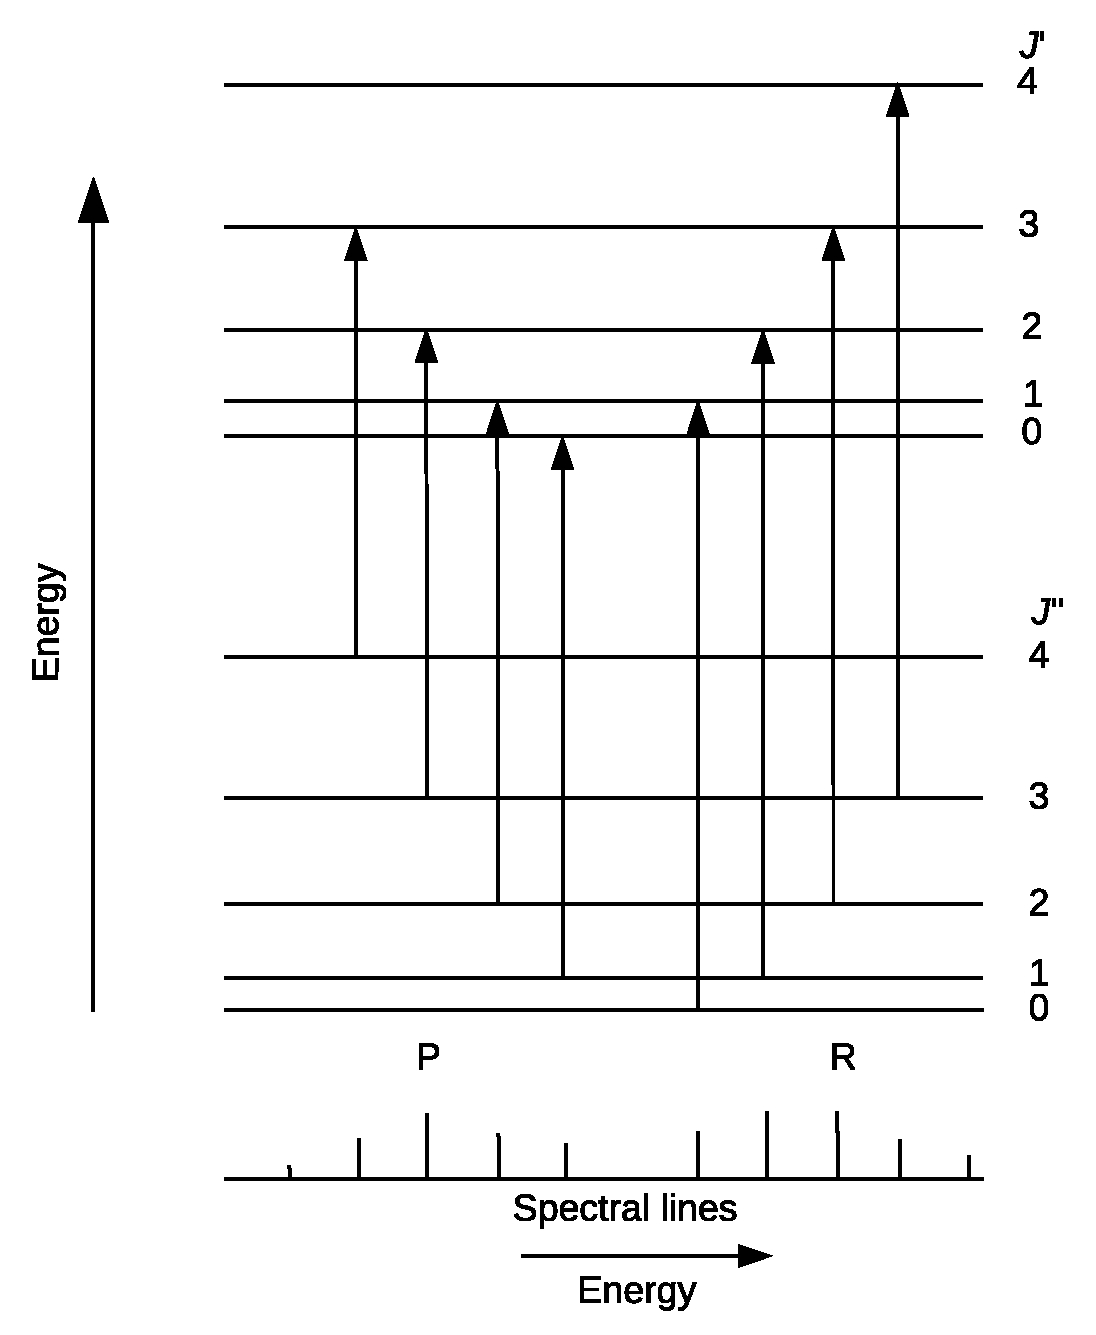
\includegraphics[scale=0.4]{fig2}
\caption{Allowed rotation-vibration transitions in a diatomic molecule. Here ($v$'', $J$'') denote the initial state and ($v$', $J$') the final state. The lower panel shows the expected rotation-vibration (IR) spectrum. The labels P and R refer to the rotational band branches.}
\label{fig2}
\end{center}
\end{figure}

The spectrum at the bottom of Fig. \ref{fig2} can be thought of having the vibrational transition at the middle, which has been split by the rotational fine structure. Two branches can be observed, which have been labeled P and R, in the spectrum. The P branch corresponds to transitions where $J$ decreases by one and R to transitions where $J$ increases by one. Note that the transitions, where $J$ does not change, are not allowed here. Only molecules that have an extra source of angular momentum, such the NO radical ($^2\Pi$ term symbol), may display $\Delta J = 0$ transitions (Q branch). Another interesting thing to note is that many
of the transitions involve rotationally excited states and in order to observe transitions originating from these states, it is necessary to have them thermally populated. As such, their intensity must depend on thermal population of the level. According to the Fermi golden rule, the intensity has the following dependency on $J$ (prime denotes the difference in vibrational states):

\begin{align}
\label{eq17}
& I_P(J) \propto \tilde{\nu}N_J^P\left|\left<\psi_J\left|H_1\right|\psi'_{J-1}\right>\right|^2\textnormal{ where }J=1,2,3...\textnormal{ (the initial rotational state)}\\
\notag
& I_R(J) \propto \tilde{\nu}N_J^R\left|\left<\psi_J\left|H_1\right|\psi'_{J+1}\right>\right|^2\textnormal{ where }J=0,1,2...\textnormal{ (the initial rotational state)}
\notag
\end{align}

\noindent
where $N_J^P$ and $N_J^R$ are the thermal (Boltzmann) populations of the initial states (including degeneracy) and $\tilde{\nu}$ is the transition energy and the last term on the right is the matrix element connecting the rotational states (the vibrational part is the same for all of the lines and does not affect the intensities). Note that each rotational level is $(2J + 1)$ -fold degenerate (i.e., that many levels with exactly the same energy). It can be shown that Eq. (\ref{eq17}) can be written as follows \cite{HERZBERG1}:

\begin{align}
\label{eq18}
& I_P(J) \propto \tilde{\nu}Je^{-\frac{\tilde{B}hcJ(J+1)}{k_BT}}\textnormal{ where }J=1,2,3...\\
\notag
& I_R(J) \propto \tilde{\nu}(J+1)e^{-\frac{\tilde{B}hcJ(J+1)}{k_BT}}\textnormal{ where }J=0,1,2...
\end{align}

\noindent
Note that here $k_B$ denotes the Boltzmann constant. This expression can be used to understand the intensity distribution of both the P and R branches, which follow essentially the thermal populations of the initial states. Note that sometimes the following notation is used for states involved in a transition: $J''$ denotes the initial state and $J'$ the final state (similar notation is also used for the vibrational quantum number $v$). By using Eq. (\ref{eq18}) and the intensity distribution of the rotational lines, the rotational temperature of the molecules can be determined (``molecular thermometer''). In practice near room temperature, it is useful to calculate the ratio between $I_P(1)$ and $I_R(1)$:

\begin{equation}
\frac{I_P(1)}{I_R(0)} = e^{-\frac{2\tilde{B}hc}{k_BT}} \Rightarrow T = -\frac{2\tilde{B}hc}{k_B\ln\left(I_P(1)/I_R(0)\right)}
\label{eq18a}
\end{equation}

\noindent
Note that at high $T$, it may be difficult to determine the intensities with high accuracy. At toom temperature, the
ratio $I_P(1) / I_R(0) \approx 0.9$.

In many cases Eq. (\ref{eq16}) is not sufficiently accurate because it does not allow for coupling of the vibrational and rotational motion. In other words, the rotational constant may be slightly different for the ground and the excited vibrational states. If the rotational constant for the lowest vibrational level (i.e., $v = 0$) is denoted by $\tilde{B}$ and for the next level ($v = 1$) by $\tilde{B}_1$, the equation corresponding to Eq. (\ref{eq16}) can be written as follows \cite{ATKINS1}:

\begin{align}
\label{eq19}
& \Delta \tilde{E}_P(J) = \tilde{\nu} - \left(\tilde{B} + \tilde{B}_1\right)J + \left(\tilde{B}_1 - \tilde{B}\right)J^2\textnormal{ where }J=1,2,3...\\
\notag
& \Delta \tilde{E}_R(J) = \tilde{\nu} + \left(\tilde{B} + \tilde{B}_1\right)(J+1) + \left(\tilde{B}_1 - \tilde{B}\right)(J+1)^2\textnormal{ where }J=0,1,2...
\end{align}

\noindent
Note that if $\tilde{B} = \tilde{B}_1$, this equation reduces to that of Eq. (\ref{eq16}). For more formal justification of using Eq. (\ref{eq19}), see Ref. \cite{HERZBERG1}. For spectral analysis, the following formulas are useful for obtaining values for $\tilde{B}$ and $\tilde{B}_1$:

\begin{align}
\label{eq20}
& \Delta\tilde{E}_R(J - 1) - \Delta\tilde{E}_P(J+1) = 4\tilde{B}\left(J + \frac{1}{2}\right)\\
\notag
& \Delta\tilde{E}_R(J) - \Delta\tilde{E}_P(J) = 4\tilde{B}_1\left(J + \frac{1}{2}\right)
\end{align}

\section{IR Spectroscopy}

In an IR experiment, the IR beam passes though the sample and photons, with energy matching the transition energy given by Eq. (\ref{eq19}), will be absorbed. The amount of absorbed light will be measured. A typical IR spectrum is shown in Fig. \ref{fig3} and a schematic overview of a Fourier Transform IR (FTIR) spectrometer is given in Fig. \ref{fig4}.

\begin{figure}[!htp]
\begin{center}
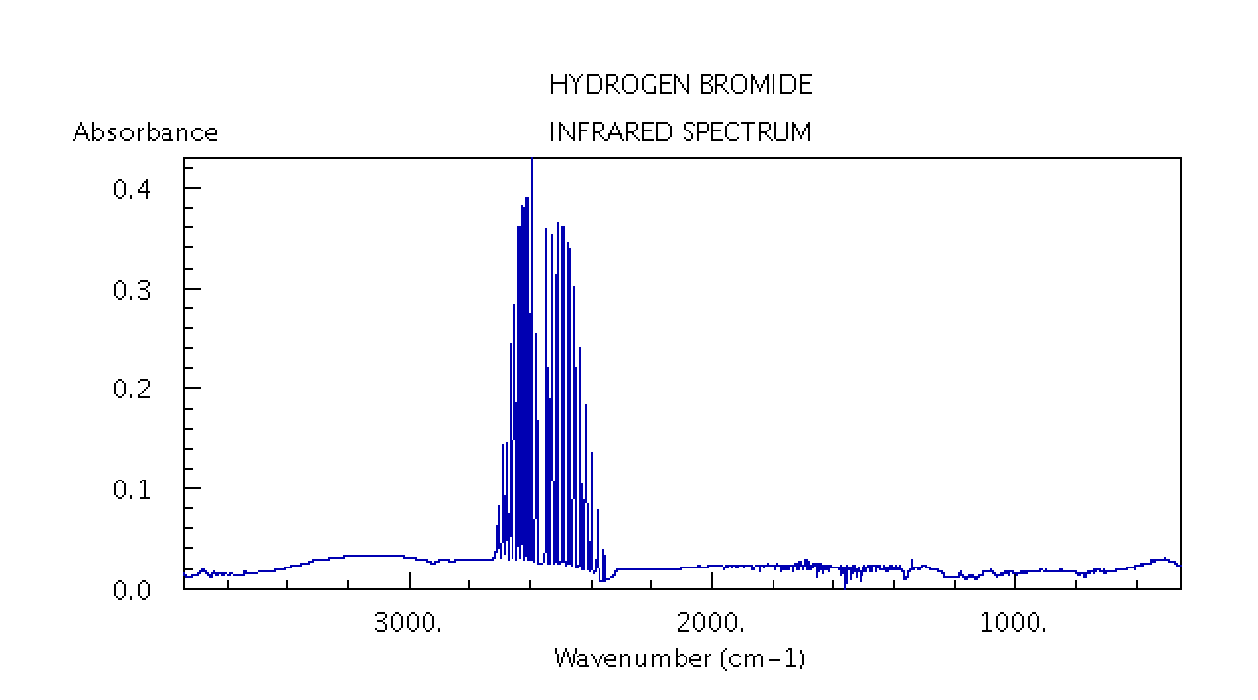
\includegraphics[scale=0.4]{fig3}
\caption{IR spectrum of HBr is shown. The $x$-axis gives the energy in wavenumber units and the y-axis indicates the amount of absorbed light \cite{webbook}.}
\label{fig3}
\end{center}
\end{figure}

\begin{figure}[!htp]
\begin{center}
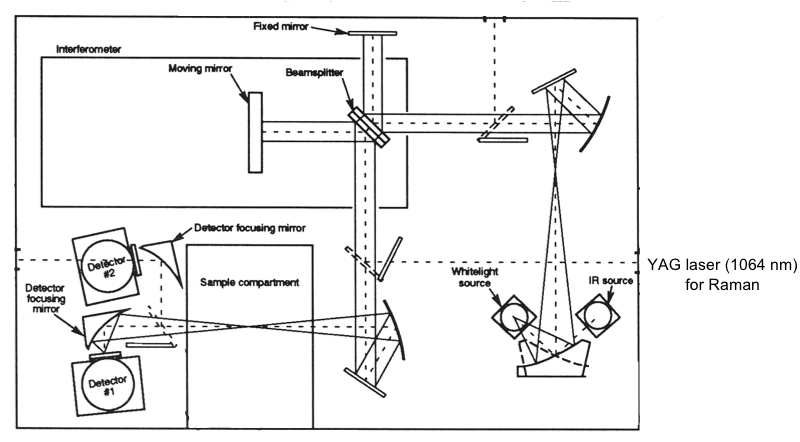
\includegraphics[scale=0.4]{fig4}
\caption{A schematic diagram of an FTIR spectrometer. Typically a heated ``glowbar'' is used as an IR light source.}
\label{fig4}
\end{center}
\end{figure}

\noindent
It is important that all the optics in the spectrometer is transparent and the applied detector is sensitive in the wavelength region relevant to the experiment. Transparent regions for some common materials are shown in Table \ref{table1} and detector sensitivity data in Table \ref{table2}. Note that most IR detectors are liquid nitrogen cooled in order to reduce the thermal noise. Recall that heat is the same thing as IR radiation

\begin{table}[!htp]
\caption{Data for optical materials typically used in IR/VIS/UV spectrometers. Materials used in this work have been emphasized.}
\begin{tabular}{l@{\extracolsep{2cm}}l@{\extracolsep{2cm}}l@{\extracolsep{2cm}}l}
 & & & \\
Material & Refractive Index & Transparent window (cm$^{-1}$) & Component in FTIR\\
BK-7 glass  &   1.5      &        4,300 -- 31,000\\
CaF$_2$     &   1.4      &        1,300 -- 66,000\\
CsBr        &   1.7      &        250 -- 33,000\\
CsI         &   1.7      &        150 -- 33,000\\
Crystal quartz& 1.5      &        3,600 -- 50,000\\
LiF         &   1.3      &        1,500 -- 90,000\\
\textbf{KBr}         &   \textbf{1.5}      &        \textbf{400 -- 33,000}      &        \textbf{Beam splitter}\\
KCl         &   1.5      &        500 -- 33,000\\
\textbf{NaCl}        &   \textbf{1.5}      &        \textbf{700 -- 28,000}      &        \textbf{Gas cell}\\
\end{tabular}
\label{table1}
\end{table}

\begin{table}[!htp]
\caption{Commonly used IR and Raman detectors. Components used here are emphasized.}
\begin{tabular}{l@{\extracolsep{2cm}}l@{\extracolsep{2cm}}l@{\extracolsep{2cm}}l}
 & & & \\
Detector & Range (cm$^{-1}$) & Detector & Range (cm$^{-1}$)\\
Polyethylene & 50 -- 650   &    MCT-B  & 400 -- 7,400\\
\textbf{MCT-A}   &     \textbf{720 -- 7,400} &   InGaAs & 5,400 -- 11,000\\
InSb    &     1,850 -- 10,000 & PbSe &  2,000 -- 11,000\\
\end{tabular}
\label{table2}
\end{table}

\section{Experiment}

\noindent
\underline{Sample preparation:}\\

\noindent
\begin{enumerate}
\item Prepare the vacuum line (see Fig. \ref{fig5}). Do not use excessive force when turning the valves! The vacuum line is made of glass and may break easily. A face shield must be worn when operating the glass vacuum line.

\item Initially all the valves indicated in Fig. \ref{eq5} must be closed. Remember that valves close by turning them clockwise and open counter clockwise. Do not open them too much or they will start leaking air from outside into the vacuum line. The mechanical pump must be on. Diffusion pump is not needed in this experiment (and may not be even present in the current vacuum line setup).

\item Connect the IR gas cell to the vacuum line by using UltraTorrs and a flextube. Make sure that the supporting metal tubes are installed inside the flextube before tightening the UltraTorr. Secure the gas cell in the metal rack behind the vacuum manifold. After installing the cell, open valves V6 and V15.

\item Open valves (in this order): V4, V5, V9 and V11. Observe the pressure readings in the capacitance manometer (CM) and thermocouple (TC). The CM readout should go to zero and the TC reading should go to about 10 mTorr (the gauge is not very accurate in this pressure region and the true pressure is lower than this). You may have to wait for up to 30 minutes for the pressure to stabilize.

\item Make sure that the HCl gas (99\% purity) is connected to the vacuum line (red gas cylinder; permanent installation).

\item[] \textbf{Warning: The gas cylinder contains pure HCl gas, which is very corrosive and poisonous!}

\item[] \vspace{0.5cm}\underline{\textbf{\Large The instructor must be present before you proceed.}}\vspace{0.5cm}

\item Open the valves (in this order): V8 and V13. Leave the system pumping for a while (up to 30 minuts). The CM readout should go to zero and TC to about 10 mTorr. If not, the tubing connecting the HCl gas cylinder and the vacuum line leaks and must be checked for leaks before proceeding.

\item Be very careful: valves V13 and V14 must never be open at the same time!

\item First close V13. Open valve V14 briefly and close it. Now you have HCl gas between the valves V13 and V14.

\item Close valves: V5 and V11. Now the vacuum line is no longer being pumped and the TC pressure sensor is protected from HCl gas.

\item Turn valve V13 very carefully and observe the reading on the CM pressure sensor. You need about 40 Torr of HCl in the vacuum line.

\item Keep V13 and V14 closed and close V15. You now have HCl gas in the IR gas cell (and everywhere in the vacuum line too).

\item Be careful with glass Dewar flasks -- under some rare circumstances they may break and shoot pieces of glass around. You must wear a faceshield when using glass Dewar flasks! Fill the Dewar flask with liquid nitrogen (L-N$_2$) and install it in place as shown in Fig. \ref{fig5}. If there are leaks in the vacuum line, it is possible that liquid air condenses in the cold trap. If the liquid air is warmed above its boiling point, it may result in rapid increase in pressure inside the vacuum line and cause explosion! Make sure you have enough L-N$_2$ in the trap during the experiment (i.e., until you have emptied the gas cell).

\item Make sure that V14 is closed. Empty the vacuum line from HCl gas by slowly opening V5. When the CM pressure display reaches zero, open very slowly V13. This
empties the HCl gas trapped between valves V13 and V14. The HCl gas will now condense into the cold trap.

\end{enumerate}

\begin{figure}[!htp]
\begin{center}
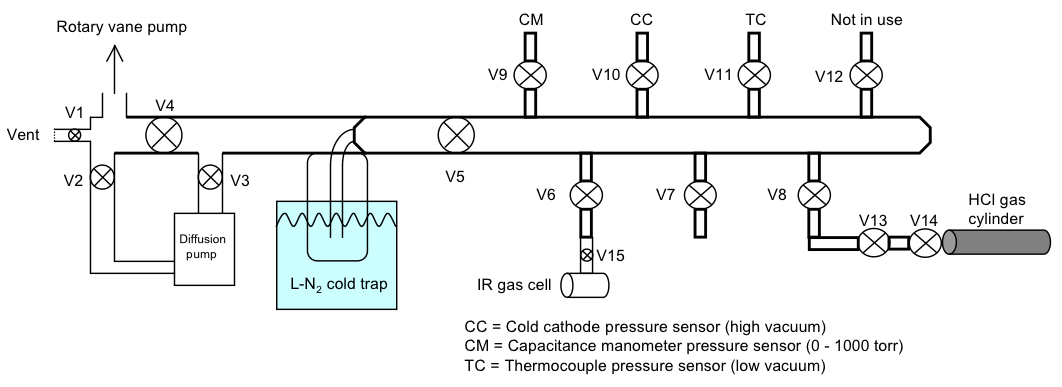
\includegraphics[scale=0.6]{fig5}
\caption{A schematic view of the vacuum line. An HCl gas bottle is connected to the inlet at V8. The bottle has two valves: the main valve (V14) and the additional valve for evacuating the connecting tube (V13). Valve V15 is installed in the IR gas cell.}
\label{fig5}
\end{center}
\end{figure}

\noindent
\underline{Emptying the IR gas cell:}\\

\begin{enumerate}
\item Connect the IR gas cell to the vacuum line with the UltraTorr and flextube. Be sure that valves V4 and V5 are open.
\item Open V6 and after that V15. Pump for 5 minutes.
\item Close valves V6 and V15.
\item Remove the IR gas cell from the vacuum line.
\item Close V4 and slowly leak air into the vacuum line through V7.
\item Remove the Dewar flask and detach the cold trap tube. Transfer the cold trap tube rapidly to a hood and leave it there until all HCl has evaporated. Keep the hood closed.After some 20 min., install the tube back into the vacuum line and continue with the last step.
\item Close V7 and open V5 slowly to evacuate the vacuum line again.
\end{enumerate}

\noindent
\underline{Measurement of the IR spectrum:}\\

\begin{enumerate}
\item Make sure that the MCT detector has liquid nitrogen in it and that the detector has cooled down. If liquid nitrogen needs to be added, fill a Dewar flask with liquid nitrogen from the tank outside and use the funnel to pour it into the detector (left side of the sample compartment). Handle liquid nitrogen with care and do not spill it on the spectrometer! It is very cold liquid (77 K; -196 $^\textnormal{o}$C; -321 F) and can cause cold burns on your skin. Use the provided stainless steel Dewar flask. \textbf{Wool gloves and a face shield must be worn when handling liquid nitrogen.}

\item \underline{The spectrometer is on at all times}, only the computer and the monitor needs to be turned on.

\item Make sure that the correct beam splitter is installed (KBr) inside the spectrometer. You can this check by opening the top lid in the spectrometer. If you need to change the beam splitter: turn the handle to release the beam splitter, put it aside into the holder, insert the new beam splitter in place, turn the handle to secure it, and close the lid.

\item If the Omnic program is not running, start it by clicking on its icon on the desktop.

\item Make sure that the Raman option (``Use Raman Accessory'') is unchecked in the ``Raman'' menu.

\item Select ``Collect $\rightarrow$ Collect Setup''. Set the number of scans to 20 and resolution to 1 cm$^{-1}$. Leave the other options as they are. Accept the changes by clicking ``OK''.

\item Select ``Collect $\rightarrow$ Optical Bench Setup''. Make sure that the settings are as follows: Sample Compartment: Main, Detector: MCT/A, Source: IR, Beamsplitter: KBr, Aperture: 32, Velocity: 1.9, check the single beam setting box, Gain: Autogain, Spectral range: 2500 -- 3200 cm$^{-1}$. If measuring the first IR sample, click on ``Align Bench'' to adjust the optics inside the spectrometer. Finally, hit ``OK''.

\item Collect the background spectrum (without the sample!) by choosing ``Collect $\rightarrow$ Collect Background''.

\item Open the sample compartment (left side of the spectrometer) and insert the sample into the IR sample holder inside the spectrometer. Center the sample along the IR beam path, which passes through the center of the sample compartment. Close the sample compartment.

\item Measure the IR spectrum by selecting ``Collect $\rightarrow$ Collect Sample''.

\item Save the spectrum on a floppy disk by choosing ``File $\rightarrow$ Save As''. Change the file type from SPA to CSV, choose the ``A:'' drive, give a filename and hit ``OK''.

\end{enumerate}

\section{Data analysis}

Read line positions and intensities for each line in the spectrum and label the lines by the Cl atom isotope (i.e., $^{35}$Cl or $^{37}$Cl), branch symbol (i.e., P or R) and the initial rotational state $J$ value. Remember that the initial state $J$ values begin from 1 for P branch and 0 for R branch. Print the IR spectrum. Extract the following from the IR spectrum:

\begin{enumerate}

\item Rotational constants $\tilde{B}$ and $\tilde{B}_1$. Use Eq. (\ref{eq20}) to calculate differences between the lines and obtain values for the rotational constants. Calculate average value for both H$^{35}$Cl and H$^{37}$Cl. Use Eq. (\ref{eq19}) for some arbitrarily chosen peak to obtain a value for $\tilde{\nu}$.

\item Use Eq. (\ref{eq18a}) to obtain the rotational temperature of the molecule.

\end{enumerate}

\section{Written laboratory report}

Follow the general instructions for written laboratory reports. The ``Results'' section must include a copy of the IR spectrum (each peak must be labeled) and the following information for both H$^{35}$Cl and H$^{37}$Cl: a list of peaks in the P and R branches, vibrational frequencies $\tilde{\nu}$, rotational constants $\tilde{B}$ and $\tilde{B}_1$, HCl bond length $r_e$ for the lowest vibrational state (Eqs. (\ref{eq14}) and (\ref{eq15})), and the rotational temperature. Provide also the literature values for $\tilde{\nu}$ and $r_e$.

\section{References}

\bibliography{../references}

\end{document}
